%   *******************************************************************
%   * THIS IS THE MAIN FILE--RUNNING LATEX ON "AllegThesis.tex" WILL  *
%   * GENERATE THE ENTIRE THESIS (ASSUMING YOU HAVE NOT RENAMED IT).  *
%   * IF YOU ARE USING BIBTEX, RUNNING BIBTEX ON "AllegThesis" SHOULD *
%   * GENERATE YOUR BIBLIOGRAPHY. SPECIFIC DETAILS DEPEND ON WHAT     *
%   * ENVIRONMENT AND TOOLS YOU ARE USING (E.G., TEXMAKER OR COMMAND  *
%   * LINE TOOLS LIKE PDFLATEX OR ...).                               *
%   *******************************************************************
%
% AllegThesis.tex
% by A. Thall
% 13 Feb 2003
%
% Revised by R. Roos
% Nov 2013
%
% This document provides a sample Senior Thesis template for use
% by students in Allegheny's CS and Applied Computing programs.
%
%   *******************************************************************
%   * LOOK FOR BLOCK COMMENTS SUCH AS THIS ONE FOR AN EXPLANATION OF  *
%   * THIS DOCUMENT AND HOW TO MODIFY IT FOR YOUR OWN THESIS!         *
%   *                                                                 *
%   * ANY LINE BEGINNING WITH A "%" IS A LATEX COMMENT AND IS IGNORED *
%   * BY THE LATEX PROCESSOR. YOU ARE ENCOURAGED TO COMMENT YOUR OWN  *
%   * LATEX CODE TO HELP YOU REMEMBER WHY YOU DID THINGS A CERTAIN WAY*
%   *******************************************************************
%

%   ********************************************************************
%   * THE FIRST SECTION OF THE MAIN LATEX FILE IS THE "PREAMBLE." IT   *
%   * INSTRUCTS LATEX TO IMPORT SPECIAL PACKAGES FOR THINGS LIKE       *
%   * INCLUDING FIGURES, DOUBLE-SPACING, COLORED TEXT, ETC.            *
%   * DEPENDING ON YOUR NEEDS, YOU MAY FIND IT NECESSARY TO USE PACK-  *
%   * AGES THAT ARE NOT INCLUDED IN THIS TEMPLATE. SIMPLY IMITATE THE  *
%   * "\usepackage{...}" COMMANDS SHOWN BELOW.                         *
%   ********************************************************************

%   ********************************************************************
%   * BEGINNING OF PREAMBLE:                                           *
%   ********************************************************************

\NeedsTeXFormat{LaTeX2e}
\documentclass[12pt]{report}

%   ********************************************************************
%   * ALL BUT ONE OF THE FOLLOWING 5 LINES SHOULD BE COMMENTED OUT.    *
%   * (NOT ALL OF THESE OPTIONS HAVE BEEN TESTED IN THIS REVISION!)    *
%   ********************************************************************

%\usepackage[debug,draft,double]{gatorthesis} % for student proof doublespace
\usepackage[bottom,double]{gatorthesis} % for final department copy
%\usepackage[debug,draft,single]{gatorthesis} % for student workcopy
%\usepackage[single]{gatorthesis} % for student
%\usepackage[debug,draft,nolists,nofront,single]{gatorthesis} % more options

\usepackage{listings}
\usepackage{comment}     % provides a way to "comment out" sections in blocks
\usepackage{doublespace} % final document should be double-spaced!
\usepackage{amsmath}     % special symbols
\usepackage{amssymb}     % more special symbols
\usepackage{epsfig}      % needed for including figures
% \usepackage{fancybox}  % --- DISABLED BY RSR, SEP 2013 ---
\usepackage[hyphens]{url}
%\usepackage{setspace}
\usepackage[figure]{algorithm2e}
\usepackage{graphicx}
\usepackage{float}
%\usepackage{tikz}
\usepackage{listings}
%\usepackage{color}
%\usepackage{tikzpagenodes}
%\usepackage{lipsum}
%\usepackage{capt-of}
%\usepackage{floatrow}
%\usepackage{subfig}
%\usepackage[latin1]{inputenc}
%\usepackage{tikz}
%\usetikzlibrary{calc,trees,positioning,arrows,chains,shapes.geometric,%
    %decorations.pathreplacing,decorations.pathmorphing,shapes,%
    %matrix,shapes.symbols,fit}
    
%\tikzstyle{decision} = [diamond, draw, fill=blue!20, 
    %text width=4.5em, text badly centered, node distance=3cm, inner sep=0pt]
%\tikzstyle{block} = [rectangle, draw, fill=blue!20, 
    %text width=5em, text centered, rounded corners, minimum height=4em]
%\tikzstyle{line} = [draw, -latex']
%\tikzstyle{cloud} = [draw, ellipse,fill=red!20, node distance=3cm,
    %minimum height=2em]

%\tikzset{
%>=stealth',
 % punktchain/.style={
  %  rectangle, 
   % rounded corners, 
    % fill=black!10,
   % draw=orange, very thick,
   % text width=10em, 
   % minimum height=1em, 
   % text centered, 
   % on chain},
  %line/.style={draw, thick, <-},
  %element/.style={
   % tape,
    %top color=white,
    %bottom color=blue!50!black!60!,
   %minimum width=8em,
    %draw=blue!40!black!90, very thick,
    %text width=10em, 
    %minimum height=1em, 
    %text centered, 
    %on chain},
  %every join/.style={->, thick,shorten >=1pt},
  %decoration={brace},
  %tuborg/.style={decorate},
  %tubnode/.style={midway, right=2pt},
%}




%   ********************************************************************
%   * OPTIONAL: IF YOU WANT VERY FINE CONTROL OVER HOW LATEX HYPHENATES*
%   * CERTAIN WORDS, YOU CAN PUT WORDS IN A "\hyphenation" COMMAND AS  *
%   * SHOWN IN THE FOLLOWING EXAMPLE. OTHERWISE, YOU MAY JUST IGNORE   *As a programmer, it is inevitable to encounter logic based based and it is imperative to be able to fix these issues. One approach to this situation is to find tools that detects these bugs. Tools will assist programmers so they can spend time on different parts of a project rather than trying to find a bug. This paper presents an empirical study to further examine the tools FindBugs, PMD, and Checkstyle used to find logic based bugs in the Java programming language.
%   * THE NEXT COMMAND.                                                *
%   ********************************************************************

% EXAMPLE: Don't hyphenate the words "itself" or "linear". Hyphenate 
%          "representations" only at the places indicated by the "-":

\hyphenation{itself repre-sen-tations linear}

%   ********************************************************************
%   * THE FOLLOWING COMMAND HAS BEEN DISABLED--IGNORE.                 *
%   ********************************************************************
% The following provides a box to surround the thesis statement
%\newenvironment{Thesis}%
%{\begin{Sbox}\begin{minipage}{.95\linewidth}}%
%{\end{minipage}\end{Sbox}\begin{center}\fbox{\TheSbox}\end{center}}

%   ********************************************************************
%   ********************************************************************
%   ***  END OF PREAMBLE.                                            ***
%   ********************************************************************
%   ********************************************************************



%   ********************************************************************
%   * DOCUMENT CONTENT STARTS AT THE "\begin{document}" COMMAND:       *
%   ********************************************************************

\begin{document}

%   ********************************************************************
%   * FILL IN THE "{...}" BELOW WITH YOUR INFORMATION.                 *
%   ********************************************************************

\thesistitle{Empirical Study of Tools to Assist Java Programmers in Finding Bugs}

\thesisauthor{Andreas Bach Landgrebe} \thesisadvisor{Professor John Wenskovitch}

\thesisnumber{CS2016-08} % SEE PAULINE LANZINE TO GET YOUR REPORT NUMBER!

\thesisreadera{Dr. Gregory M. Kapfhammer}


%   ********************************************************************
%   * IN RARE CASES YOU MAY HAVE MORE THAN TWO READERS, IN WHICH CASE  *
%   * YOU SHOULD UN-COMMENT THE FOLLOWING AND ADD NAMES:               *
%   ********************************************************************
% \thesisreaderb{Dr. Your Thirdreader} 
% \thesisreaderc{Dr. Your Fourthreader}
% \thesisreaderd{Dr. Your Fifthreader}

%   ********************************************************************
%   * YOU MAY IGNORE THE FOLLOWING COMMAND:                            *
%   ********************************************************************
\date{\FileRevised \\ $\mbox{}$Revision: 1.8 $\mbox{}$}

\thesismaketitle         % Creates the title page
\thesismakecopyright     % Creates the copyright page

%   ********************************************************************
%   * YOU MAY SPLIT YOUR THESIS INTO SEVERAL FILES AND "\include" THEM *
%   * AS SHOWN BELOW. FOR INSTANCE, FILE "abstract.tex" CONTAINS THE   *
%   * ABSTRACT, FILE "ack.tex" CONTAINS THE ACKNOWLEDGMENTS, ETC. YOU  *
%   * MAY, OF COURSE, PUT EVERYTHING INTO ONE HUGE FILE, BUT THERE ARE *
%   * ADVANTAGES TO SPLITTING THINGS UP--FOR EXAMPLE, YOU CAN COMMENT  *
%   * OUT "\include" LINES OF SOME PARTS IN ORDER TO PRINT DRAFTS      *
%   * CONTAINING SELECTED SECTIONS OF YOUR THESIS, SAVING PAPER AND    *
%   * PRINTING COSTS.                                                  *
%   *                                                                  *
%   * YOU ARE NOT REQUIRED TO HAVE A "dedication"--IF YOU DON'T, JUST  *
%   * DELETE THAT LINE OR COMMENT IT OUT WITH A LEADING "%"            *
%   ********************************************************************

\begin{abstract}
As a programmer, it is inevitable to encounter logic based bugs and it is imperative to be able to fix the issues. One approach to this situation is to use tools that helps detect logic bugs. Tools can assist programmers to find logic errors so they can spend time on different tasks in their projects. This paper presents an empirical study to examine three tools FindBugs, PMD, and Checkstyle used to find logic based bugs in Java programs.
\end{abstract}
  % REQUIRED!

%\include{dedication} % OPTIONAL

\chapter*{Acknowledgment}\label{ch:ack}
\addcontentsline{tob}{section}{Acknowledgment}

I like to acknowledge:

\begin{enumerate}


\item[]
Prof. John Wenskovitch, for continuing advice and support, and for relentlessly forcing me to do my best.

\item[]
Dr. Gregory M. Kapfhammer, for continuing advice and support as a mentor and a professor.

\item[]
Dr. Robert Cupper, for starting me on the path I follow today.

\item[]
Every other member of the Allegheny faculty, for unparalleled excellence throughout my education.

\item[]
My colleagues, for advice, support, and patience throughout my Allegheny career.

\item[]
To all of the students who took time out of their busy schedule to participate in my empirical study

\end{enumerate}       % OPTIONAL, BUT ALMOST EVERYONE INCLUDES IT

%   ********************************************************************
%   * FRONT MATTER--TABLE OF CONTENTS, ETC. YOU PROBABLY DON'T NEED TO *
%   * CHANGE ANY OF THIS UNLESS YOU HAVE NO TABLES OR FIGURES, OR YOU  *
%   * WANT TO CHANGE NUMBERING DEPTH FOR SUBSECTIONS, OR ...           *
%   ********************************************************************

\setcounter{tocdepth}{2}    % # of section levels shown in table of contents
\setcounter{secnumdepth}{3} % # of numbered subsection levels in the text

\tableofcontents
%\listoftables       % OMIT THIS IF YOU DON'T HAVE ANY TABLES
\listoffigures      % OMIT THIS IF YOU DON'T HAVE ANY FIGURES

%   ********************************************************************
%   * A GLOSSARY IS ALMOST NEVER NEEDED UNLESS YOU HAVE AN UNUSUALLY   *
%   * LARGE NUMBER OF SPECIAL TERMS OR NOTATIONS AND IT WOULD DETRACT  *
%   * TOO MUCH FROM THE FLOW OF THE PAPER TO DEFINE THEM IN-LINE.      *
%   ********************************************************************
%\include{glossary}  % OMIT THIS IF YOU DON'T HAVE A GLOSSARY (FEW PEOPLE DO)


%   ********************************************************************
%   * THE FOLLOWING "lstset" COMMAND IS ADAPTED FROM ONE FOUND AT:     *
%   * http://tex.stackexchange.com/questions/115467/                   *
%   * listings-highlight-java-annotations                              *
%   *                                                                  *
%   * SEE CHAPTER 3 AND APPENDIX A                                     *
%   ********************************************************************

\lstset{
  basicstyle=\footnotesize\tt, % the size of the fonts that are used for the code
  breakatwhitespace=false,     % automatic breaks only happen at whitespace?
  breaklines=true,             % sets automatic line breaking
  captionpos=b,                % sets the caption-position to bottom
  frame=single,                % adds a frame around the code
  language=Java,               % the language of the code
  keywordstyle=\bf,
  showspaces=false,
  showstringspaces=false,      % underline spaces within strings only?
  showtabs=false,
  tabsize=2                    % sets default tabsize to 2 spaces
}

%   ********************************************************************
%   * NOW INCLUDE THE CHAPTER FILES; COMMENT OUT ANY YOU DON'T WANT TO *
%   * PROCESS IN A PARTICULAR LATEX RUN.                               *
%   *                                                                  *
%   * INCLUDED FILES ARE ASSUMED TO END IN ".tex", E.G.,               *
%   * "ch01_overview.tex", "ch02_relatedwork.tex", ETC.                *
%   ********************************************************************

% ch:intro
%
% $Id: ch01_overview
%
%   *******************************************************************
%   * SEE THE MAIN FILE "AllegThesis.tex" FOR MORE INFORMATION.       *
%   *******************************************************************

\chapter{Introduction}\label{ch:intro} % we can refer to chapter by the label

%   ************************************************************************
%   * In LaTeX, new paragraphs are begun by simply leaving a blank line in *
%   * the LaTeX file.                                                      *
%   *                                                                      *
%   * The \\ characters should NEVER be used to end a paragraph.           *
%   * They are used only for inserting line breaks in certain situations.  *
%   *                                                                      *
%   * "Widows" (ending paragraph lines at the top of a new page) and       *
%   * "orphans" (opening paragraph lines at the bottom of a page) should   *
%   * be eliminated; this sometimes requires re-writing some of the        *
%   * text to change the line lengths.                                     *
%   ************************************************************************


%The purpose of this sample thesis is to show various \LaTeX\ formatting
%commands. Information about content should be obtained through consultation
%with the thesis readers and examination of past senior theses.
%There are no fixed rules governing the number of chapters or their titles---old 
%senior theses and discussions with the thesis readers are the best resources
%for making such decisions.

%Usually, a chapter begins with a paragraph or two that serves as a
%sort of mini-introduction to the chapter. This is followed
%by numbered sections created with ``\verb$\section{...}$'', 
%``\verb$\subsection{...}$'', etc.




\section{Motivation} \label{sec:motivation}
%The first paragraph in each section is not indented---that is a standard style
%that is enforced by the \LaTeX\ program. It should never be necessary to
%insert commands to force paragraph indentation.

When programmers write code in Java programming language, there is a high chance that some of the programs do not run as expected. There are many options to fix this issue. One approach is to look back into the source code and read it line-by-line and try to find out what the issue is. This approach is time consuming and tiresome and may not always work. An alternative approach is to use a tool such as FindBugs, PMD, or Checkstyle to help finding the issue.
\newpage
\begin{figure}[htbp]
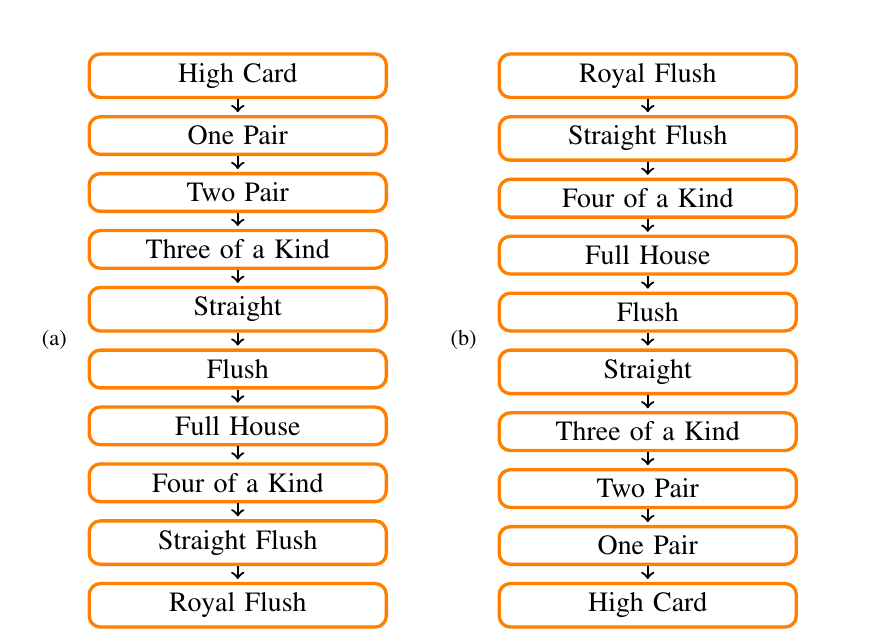
\includegraphics[scale=0.4]{motivationImproved.png}
\caption{The Figure shows the representation of poker hands - (a) starts with the lowest hand (b) starts with the highest hand. The highest hand is the winner of the game, and therefore the program code should use the representation (b) to decide the winner.}
\label{fig:pr}
\end{figure}


For example, let us say we are writing a program in Java that will decide the winner of a poker game. Figure 1.1 shows the different poker hands that a player can have. Figure 1.1 (a) shows the sequence of hands starting with the lowest hand `high card' and ending with the highest hand `royal flush', where figure 1.1 (b) starts with the highest hand `royal flush' and ends with the lowest hand `high card'.
The program is written so it looks at poker hands starting at the beginning of the representation and continues to go through the poker hands in the representation until a match between the poker hand and the representation is found. If there is a match the program will select the hand as the highest hand.
Using the representation in Figure 1.1 (a) the program will start with the `high card'. A poker hand always has a highest card so it will stop here and select the highest card as the poker hand. This is not correct because there could also be `one pair', `two pair', `three of a kind' or any of the other hands listed in the representation. Using this representation will not necessarily find the highest poker hand.      
Using the representation in Figure 1.1 (b) the program will go through the representation starting with the highest hand, and select the first match, which will give the highest hand and this is correct.

Figure 1.1: The Figure shows the representation of poker hands - (a) starts with the lowest hand and (b) starts with the highest hand. The highest hand is the winner of the game, and therefore the program code should use the representation (b) to decide the winner.  



%For example, let us say we are writing a program in Java to decide the winner of the poker game. Figure \ref{fig:pr} shows the different poker hands that a player can have. Figure \ref{fig:pr} (a) shows the sequence of hands starting with the lowest hand, `high card' and ending with the highest hand, `royal flush' where Figure \ref{fig:pr} (b) starts with the highest hand, `royal flush' and ends with the lowest hand, `high card'. The representation in Figure \ref{fig:pr} (a) would not be correct to use in the program because the program would look for a lower hand before it looks for a higher hand and therefore not select the highest possible hand. To fix this issue, the program should use the representation shown in Figure \ref{fig:pr} (b) to evaluate the winning hand of the poker game. The tools FindBugs, PMD, and Checkstyle will be evaluated to find out if they could suggest that the bug is in the sequence of the poker hand representation.   

%shows the correct representation on how to follow a game of poker. Figure \ref{fig:pr} (a) would be a wrong because a program is looking for a hand that contains a pair before they look for a hand that could possibly have two pairs inside it. Therefore this design will not select the highest possible combination. To fix this, Figure \ref{fig:pr} (b) would be the correct representation of how a game of poker should be played. The tools of FindBugs, PMD and Checkstyle will be evaluated to see if they ciouyld suggest the big is in the sequence of the poker hand representation.

%The thesis should avoid the use of second-person pronouns such as ``you''
%and ``your,'' as well as the use of imperative statements (implied
%second-person) such as ``Look
%at \ldots'' or ``Consider the following example \ldots''. 
%First person (``I,'' ``my,'' etc.) is sometimes acceptable, 
%but should be used sparingly. (This is an appropriate topic 
%or discussion with the first reader of the project.) Contractions (``don't'',
%`can't'', etc.) are considered informal and should be avoided. Common
%abbreviations such as ``math'' for ``mathematics'' or ``comp'' for 
%``senior comprehensive project''  are also informal and not appropriate
%in the final thesis.

%Figures illustrating complex or hard-to-describe concepts are essential.
%All figures should be fully explained in the text. For example,
%Figure \ref{latexprocess} shows the first step in processing a senior thesis.
%The user files consist of the main file, {\tt AllegThesis.tex}, and zero or
%ore additional files ({\tt ch01.tex}, {\tt ch02.tex} in the figure). Not shown
%n the figure are image files, the bibliography, and other included
%components (the ``\ldots etc.\ldots'' on the left side of the figure). 
%Typing the command {\tt pdflatex} with the main file name
%produces a number of additional files, including an {\tt .aux} file (with
%information such a label references and citations),
%a table of contents, or {\tt .toc}, file, a printable {\tt .pdf} file, and
%a number of others, depending on the document.

%   *******************************************************************
%   * FIGURES ARE PLACED ACCORDING TO A SET OF CONSTRAINTS THAT CAN   *
%   * BE MANIPULATED TO SOME DEGREE.                                  *
%   * A SEARCH FOR "controlling latex floats" TURNS UP A NUMBER OF    *
%   * SITES THAT HAVE USEFUL INFORMATION, FOR EXAMPLE:                *
%   *                                                                 *
%   * http://mintaka.sdsu.edu/GF/bibliog/latex/floats.html            *
%   * http://goo.gl/aC8E8Q                                            *
%   * http://robjhyndman.com/hyndsight/latex-floats/                  *
%   *******************************************************************

%\begin{figure}[htbp]
%\centering
%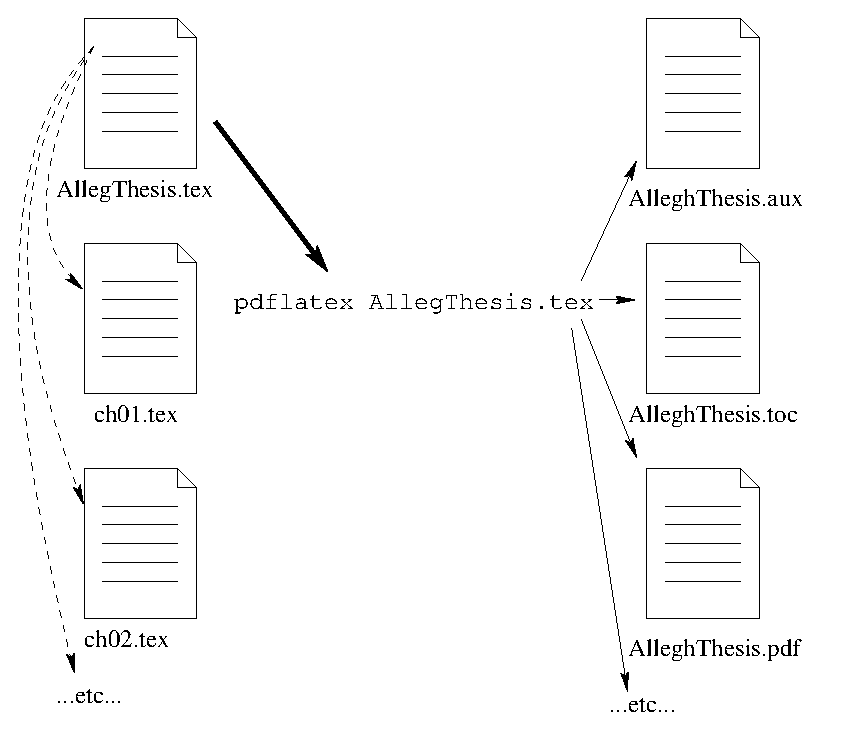
\includegraphics[width=3.5in]{latexprocess}
%\caption{The first step in creating a thesis document}
%\label{latexprocess}
%\end{figure}

\section{Current State of the Art}\label{sec:stateofart}
%There are multiple
%ways to create {\it italicized}, {\bf bold-face}, {\tt fixed-width}, and
%{\sf sans-serif} fonts, as well as combinations, e.g., \textit{\textbf{
%bold italic}} or \textit{\textsf{italic sans-serif}}. The \LaTeX\ source
%file for this chapter shows some of the ways to achieve these effects.
%It is customary to use fixed-width font for program constructs, e.g.,
%`In the Java code accompanying the figure, {\tt n} stands for the 
%umber of generations to be simulated by the {\tt evolvePopulation()} method.'' 
%Variables in mathematical equations are normally rendered in 
%talics, e.g., ``In the performance equation, {\it cpuTime} is 
%the average time over fifty runs of the program.''

%It is the privilege of the thesis author (in consultation with the
%project super(a) shows the wrong representation and (b) shows the correct representation to follow when playing a game of pokervisor and other readers) to decide on the best way to 
%organize the sections and chapters in the way that makes the most sense.
%If the introduction begins with a motivating
%anecdote, perhaps this is best followed by defining a few terms or mentioning
%some major results that the reader should be aware of right from the 
%beginning. But 
%It is important to get as quickly as possible to 
%a concise statement of the {\it thesis}---the main question 
%addressed by the project. This might merit a separate
%ection of the chapter.

At present, the process of locating logic based bugs is mostly manual. However, there are tools to assist in finding logic based bugs. Many of these tools have been developed using techniques such as syntactic pattern matching, data flow analysis, type systems, model checking, and theorem proving \cite{bugFindingTools}.


\section{Definitions}\label{sec:definitions}
 logic based bug is defined as a bug in a program that causes it to operate incorrectly. The program will not terminate abnormally or crash. This is considered to be fault of commission. An example of a logic based bug is comparing String objects with the == operator compared to the .equals() method. When it comes to objects, when using the == operator, it is testing for references equality. This means that it is checking if the two are the same object. The .equals() method tests for value equality. This means that it is testing if the two objects are logically ``equal". 
 
 
 %An example of a logic based bug when you have a program that is supposed to calculate velocity squared. Velocity squared should equal $2 * (kinetic / mass).$ But instead, your program is calculating Velocity squared to be $3 * (kinetic / mass).$ Due to the fact that the program does not follow the law of physics, this is considered to be a logic based bug. 
 
Source code analysis is defined as: ``Source code analysis is the process of extracting information about a program from its source code or artifacts generated from the source code using automatic tools" \cite{Binkley}. The idea of source code analysis is imperative in order to figure out how programs works. Source code analysis is also used to locate bugs in programs.
  
 Static program analysis of software is defined as analysis that is completed without actually executing programs and is usually performed as part of a Code Review. The analysis attempts to highlight possible errors within the source code. The three tools analyzed in this paper FindBugs, PMD, and Checkstyle are examples of static program analysis. These tools intend to identify errors in Java code without running the program. 
 %The tools are grouped into four types. The first group is code analysis where statements are highlighted if the syntax is wrong. logic based bugs
 %This group generates a graph from the components submitted as input. The third group is called data analyzers and reviews the data structures to identify improper linkage among components. The fourth and last group is called a sequence checker and checks the sequences of events. Events that might be coded in an incorrect sequence are highlighted.

Dynamic Program Analysis is defined as the analysis of computer software that is performed by executing programs on a real or virtual processor. Tools using Dynamic Program Analysis are also known as program monitors because they watch and report the program's behavior. 

Fault of omission is when some key aspect of the code is missing. For example, when a variable is not initialized.

Fault of commission is when there are one or more 
incorrect assignments in a program. For example, when a variable is initialized to the wrong value.

Compiler bug is defined as a bug that is detected by the compiler when compiling the source code and it prevents it from being executable. An example of a compiler bug is writing a line of source code without a semi colon (;) at the end of the statement.

 Run-time bug is defined as a bug that occurs during the execution of a program. In contrast to logic based bugs, a run-time bug will terminate or crash the program. 

 False Positive is defined as a condition that is incorrectly reported as an error. For example the tools FindBugs, PMD, or Checkstyle could report a false positive if they scan through source code and highlight lines in the code that actually do not contain any bug.  
 
 False Negative is defined as a condition where a test result improperly indicates no presence of an error. For example tools FindBugs, PMD, or Checkstyle could report a false negative if they scan through source code and fail to highlight lines of the code that actually hold bugs. 
 
 Cyclomatic Complexity is defined as a measurement used to indicate the complexity of a program. This  metric calculates the number of linearly independent paths through a program's source code. The tool PMD is able to measure the complexity of a program by calculating the number of linearly independent paths in a program's source code.

 Inefficient Code is when complex code can be re-written to be simpler. An example of inefficient code in Java is using the String.trim().length() to check if a string is empty. This approach creates a new String object just to check its size. Instead a static function that loops through the string should be used as this would be a much more efficient way to check if a string is empty. 
 
 Bug checker is defined as a static analysis tool used to find code that does not conform to specific properties and which may cause the program to misbehave at runtime \cite{bugFindingTools}. An example of a bug checker is the tool FindBugs.
 
 Style checkers examine code to determine if it contains non-conformance to particular coding style rules \cite{bugFindingTools}. Enforcing style checkers create a consistent style throughout  programs and projects. This makes it easier for developers to understand and maintain code for a particular project. Two examples of style checkers are PMD and Checkstyle.




\section{Goals of the Project}\label{sec:goals}
%This section could also be entitled ``Thesis'' or something similar. 
There are two significant goals for this project. The first goal is to perform the empirical study of the tools and this goal is a prerequisite for the second goal. The second goal is to determine whether new tools should be developed or additional features could be added to one or more of the existing tools. If none of the three tools FindBugs, PMD, and Checkstyle are successful in assisting the programmer in finding logic based bugs then it may be recommended that a new tool should be developed. However, if at least one of the three tools are able to successfully assist in locating the bugs, then the tool may be the future tool used to assist in such a tedious and time-consuming task. 
 
%A formal thesis statement should be a 
%\emph{falsifiable} % COMMENT OUT THINGS THAT YOU MAY LATER WISH TO PUT BACK
%statement about 
%the goal achieved by the project.  For a purely scientific
%project, this is the hypothesis being tested; it should be a
%\emph{falsifiable} statement, i.e., one that can be disproven through
%an appropriate experiment.
%For an applied programming project, it is usually a statement about 
%the feasibility and correctness of the approach used and the advantages it 
%has over other approaches, using suitable metrics.  For a survey or study,
%it is usually a statement regarding the need 
%or usefulness of such a study, its intended audience, and so on.

% COMMENTED OUT NEXT FEW LINES TO SAVE SPACE; MAY PUT THEM BACK LATER
%Following the concise statement of the thesis, some of the details can be
%expanded.  
%It is appropriate to
%refer to some of the results in the introduction (which may 
%mean going back and adding them to the introduction once the
%research is completed). 
%A senior thesis, or any research paper, is not a mystery 
%novel---there is no need to keep the reader in suspense about what
%has been accomplished.

\section{Thesis Outline}\label{sec:outline}
%The introductory chapter usually concludes with a ``road map'' of the upcoming
%chapters, e.g., ``Chapter \ref{ch:relatedwork} reviews a number of past approaches
%to the problem and summarizes their strengths and weaknesses. Chapter 
%\ref{ch:method} outlines the method of approach used to establish the
%results.''

This paper consists of eight chapters which cover topics for my senior project. Chapter 2 will discuss the related research work that is on-going in the field of assisting in locating logic bugs. Chapter 3, 4, and 5 will describe the three tools FindBugs, PMD, and Checkstyle accordingly including their features and functionality. Chapter 6 outlines the methodology I have used for this project including how each participant conducted the study and descriptions of the buggy programs I have developed. In chapter 7 the results of this empirical study are presented and discussed and this is used to form the conclusion. Chapter 8 is the conclusion of my study and it also includes suggestions for further studies.     
 % Introduction -- of course, you can name it anything!

% ch:relatedwork
%
% $Id: ch02_relatedwork
%
%   *******************************************************************
%   * SEE THE MAIN FILE "AllegThesis.tex" FOR MORE INFORMATION.       *
%   *******************************************************************
\chapter{Related Work}\label{ch:relatedwork}

 Automated and semi-automated analysis of source code has remained a topic of intense research for more than 30 years \cite{Binkley}. It helps programmers to work more efficiently and enforces rules to use the same programming patterns. This paper will explore and compare the effectiveness of some of these tools. In this chapter, some additional tools are mentioned 
 


\section{Java Visualizer}

\begin{figure}[htbp]
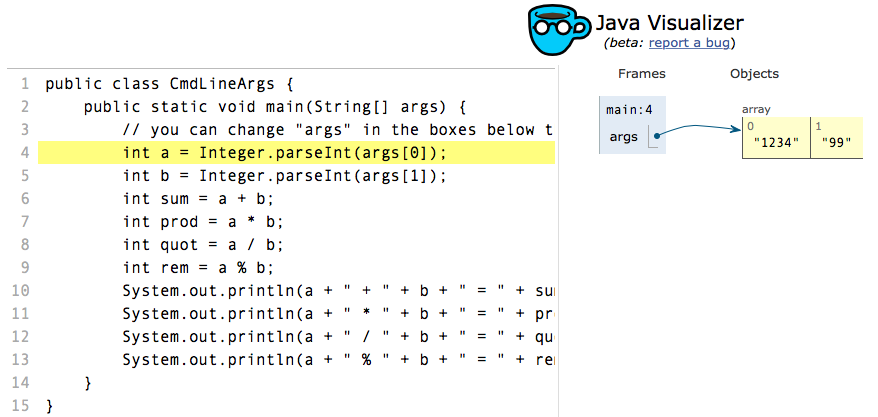
\includegraphics[scale=0.5]{JavaVisualizer}
\caption{Java Visualizer used to go through a Java program line by line}
\label{fig:jv}
\end{figure}

In Table \ref{fig:jv}, the Java Visualizer is used to go through a Java program line by line and provide a visualization of the program steps on the right hand side.

\section{Jlint}
%Jlint
Jlint is a static code analyzer that checks Java source code to attempt to find bugs. Throughout the code, it looks for inconsistencies and synchronization problems. It is done by performing data flow analysis and building a lock graph. Jlint is a simple but highly effective static analyzer that checks Java programs for several common errors, such as null pointer exceptions and overflow errors \cite{artho_havelund}.
%Applying Jlint to Space Exploration Software
The original version Jlint1 was just a Java program checker that could check packages in an automated manner. Jlint1 was extended to Jlint2 to fully support synchronization. \cite{Artho:2001:ASA:872024.872575}.
%Applying Static Analysis to Large-Scale, Multi-Threaded Java Programs
\section{Bandera}
Bandera is an integrated collection of program analysis and transformation components \cite{Corbett:2000:BEF:337180.337234}. %Bandera: Extracting Finite-state Models from Java Source Code
Bandera takes Java source code and outputs a program model in the input language for several existing verification tools \cite{Corbett:2000:BEF:337180.337234}.

Bandera evaluates the model by checking the Java source code. It provides tool to support definition and managing collections of requirements \cite{Corbett:2000:BSI:337180.337625}.
%Bandera: A Source-level Interface for Model Checking Java Programs

\section{ESC/Java2}
%ESC/Java 2
ESC/Java2 (Extended Static Checker for Java) is the main (extended) static checker for the JML (Java Modeling Language) \cite{chalin_kiniry_leavens_poll}. The purpose of the extension is to include extra constructs for specifying an object-oriented module such as frame properties, data groups, and ghost and model fields \cite{chalin_kiniry_leavens_poll}.
%Beyond Assertions: Advanced Specification and Verification with JML and ESC/Java2

At first, it was an experimental compile-time program checker that found common programming errors. The checker is powered by verification-condition generation and automatic theorem-proving techniques \cite{Flanagan:2002:ESC:512529.512558} \cite{Flanagan:2002:ESC:543552.512558}.
%Extended Static Checking for Java

\section{Summary of Related Work}
There are a number of tools that assist programmers in working more effectively. Three of these have been researched in this paper, but apart from these there are many other tools. The tools that are presented in this paper may not detect a possible bug (false negative) or may highlight a point in the source code that may not be the bug (false positive). My proposed study is to evaluate three tools for four Java programs that have been written to include a bug. This will provide Java programmers information about tools to assist in detecting logic based bugs.


%A typical second chapter deals with a survey of the literature
%related to the thesis topic. The subsections may be organized in whatever
%manner seems best suited to the material---chronological, or by topic, or
%according to some other criteria (e.g., primary versus secondary resources).
%The examples given in the sections in this chapter are nonsensical in content;
%they are provided merely to give examples of citing bibliographic references.
%Resources should be cited by author name(s), not by title.
%There should be a space between the square brackets of a citation and
%any preceding words. Thus, ``Smith and Jones[17]'' is wrong; ``Smith and
%Jones [17]'' is correct. If the citation is at the end of a sentence, the
%period goes after the brackets (``Johnson [23].'', not ``Johnson. [23]'').


%The earliest work done in widget software is described in the seminal 1986
%paper by Smith and Jones \cite{SmithJones86}. Using a networked array of
%high-performance computers they demonstrate that widgets with $k$ degrees
%of freedom can be simulated in time proportional to $k\log^2k$. At the
%heart of their demonstration is an algorithm for re-encabulating the widgets
%using a lookup table that can be updated in real time, assuming that
%the widgets are non-orthogonal. The question of simulating orthogonal widgets
%is left open, but the authors conjecture that orthogonality will add at
%ost another factor of $k$ to the performance upper bound.


%A number of papers \cite{blum67,damon:95,zobel:97} deal with issues
%that are peripheral to the orthogonal case, but Dio\c{s}an and Oltean
%were the first to tackle it directly.
%In their 2009 paper \cite{diosan09}, 
%Dio\c{s}an and Oltean apply evolutionary techniques to
%the orthogonal widget case, obtaining empirical results that suggest
%an efficient algorithm might be at hand. Their
%approach is characterized by the use of a genetic algorithm to evolve other,
%more problem-specific evolutionary algorithms. 

 % Background, literature survey, ...

% ch:method
\include{ch03_FindBugs} % Chapter organization is topic-dependent

%ch:implem
\chapter{PMD}\label{ch:pmd}

PMD is a static source code analyzer. This tool looks at Java source code and identifies bugs or potential anomalies. These anomalies include dead code, duplicated code or overcomplicated expressions \cite{Urma}.

The first version of PMD (version 0.1) was introduced in 2002. The version of PMD that was used in this project is 5.4.1. 

PMD can check for more that plain java program issues. Its rules are divided into 5 sections: jsp, xsl, java, ecmascript, and xml. In the java section there are 276 different checks divided into 16 categories: Design (52), Coupling (10), Jakarta Commons Logging (3), Basic (23), Strict Exceptions (12), Security Code Guidelines (2), Java Logging (4), Android (3), Controversial (23), Comments (3), Type Resolution(4), Empty Code(11), String and StringBuffer (15), Code Size (11), Braces (4), Unused Code (5), Unnecessary (7), J2EE (9), JavaBeans (2), Migration (14), Import Statements (6), JUnit (12), Naming (20), Finalizer (6), Optimization(12), and Clone Implementation(3). The number in parenthesis marks the number of checks in that category. The rules range from styling checks like ``ShortMethodName: Method names that are very short are not helpful to the reader" in the Naming category to rules for checking code design like ``UseSingleton: For classes that only have static methods, consider making them Singletons. Note that this doesn't apply to abstract classes, since their subclasses may well include non-static methods. Also, this class is a Singleton, a private constructor should be added to prevent instantiation."

From the rule sets PMD uses, it is able to assist programmers in finding logic based bugs. Some of the categories that may be able to identity potential bugs include Controversial, Empty Code, and String and StringBuffer. One of the rules in the category, Controversial that may cause a logic based bugs is the UnnecessaryParantheses. UnnecessaryParantheses is using the order of operation to calculate a certain math equation, and parantheses that are used may lead to an incorrect answer. In the category Empty Code, one ruleset that may lead to logic based bugs is EmptyCatchBlock. If the catch block is empty, then nothing will be done which could cause an incorrect calculation. In the category of String and StringBuffer, one ruleset that caused a logic based bug was the UseEqualsToCompareStrings. In this ruleset, if two string are compared in an if statement by using ==, this is not going to work correctly. This is because the == operator looks at what the string point to rather than the content of the strings. To fix this, the .equals() method should be used to compare two strings.

Comparing FindBugs and PMD, PMD has found to produce a larger amount of warnings than FindBugs. Despite that more warnings in a piece of source code will be generated with PMD compared to FindBugs, this does not mean that FindBugs or PMD is the better tool. These two tools focus on two different aspects of software quality \cite{Hovemeyer:2004:FBE:1028664.1028717}. PMD focus on looking at a coding style. FindBugs focuses on helping to uncover errors while ignoring style issues. Since these two tools focus on two different aspects of software quality, these two tools are complements of each other and not substitutes.

\newpage
\begin{figure}
\begin{center}
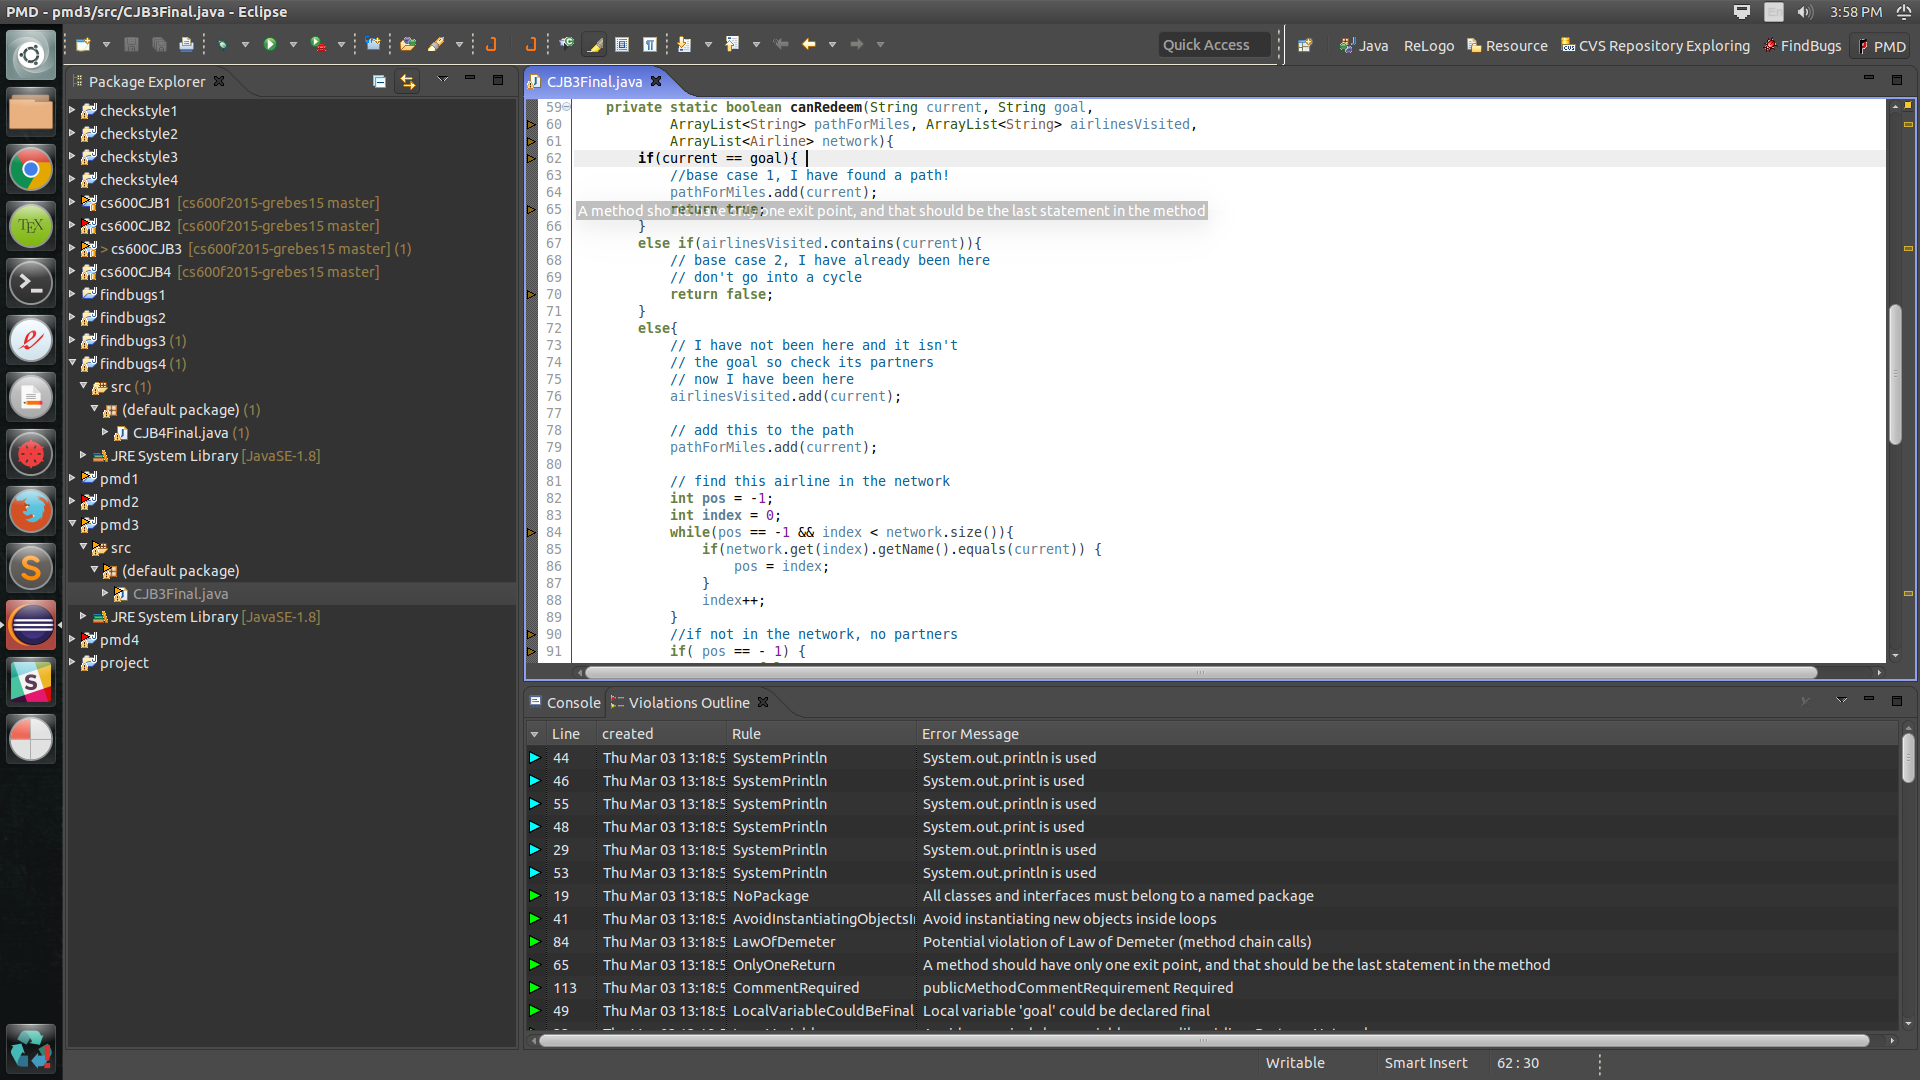
\includegraphics[width=1.15\textwidth]{pmd.png}
\end{center}
\caption{Example of PMD used in the Eclipse Integrated Development Environment}
\label{fig:pmd}
\end{figure}
Figure \ref{fig:pmd} is a screenshot taken that shows the PMD tool used in the empirical study. Inside of the Eclipse Integrated Development Environment, PMD highlights multiple lines of source code and displays a warning. All of the highlighted lines can be seen on the left side of the line numbers.   

\section{AST - Abstract Syntax Tree}
\label{sec:ast}

An Abstract Syntax Tree is an tree representation of the source code. This tree can be viewed as a structured document - just like XML. Since it is  conceptually similar to XML, it can be queried with XPath to find a pattern \cite{pmd}. By having the source code represented as a tree means the checks can be made at isolated nodes in the tree, irrespective of branches higher up and below. The Abstract Syntax Tree shows the structure of the code - the blocks and statements that are contained within each element.

\begin{figure}[H]
\begin{center}
	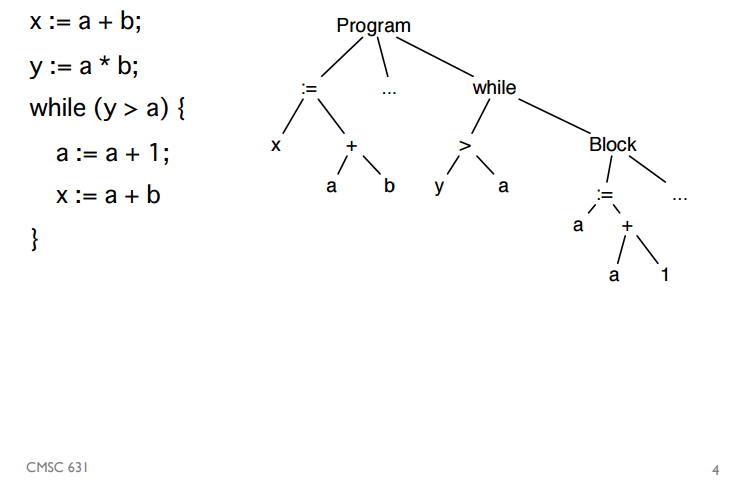
\includegraphics[width=0.9\textwidth]{image001.png}
\end{center}
\caption{Example of an Abstract Syntax Tree that both PMD and Checkstyle use. \cite{1_foster_2016}.}
\end{figure}

  % Chapter organization is topic-dependent

% YOU MAY HAVE SEVERAL MORE CHAPTERS, DEPENDING ON TOPIC AND ORGANIZATION

\include{ch05_Checkstyle}
%ch:conclusion
 % Conclusion/future work

\chapter{Methodology}\label{ch:methodology}

The next step for this senior project was to conduct an empirical study. Participants in this study have been selected among students who have had the class of Computer Science 112 or more advanced classes at Allegheny College. These students will in this paper be referred to as participants. 

Conducting the empirical study help me to determine how effective and useful the tools are. The results will tell me if participants were able to use the tools to assist them in finding logic based bugs in their code or if they were better off reading and analyzing the source code line by line to find the bugs.  
 
Ideally, the sample size should be at least 20 participants in this study. However, for practical reasons it has only been possible for me to get six students to participate and respond to my study. Therefore the results from my study cannot form the basis for a strong conclusion but rather give indications of the usefulness of the tools.  

I have developed four Java programs and each program has a bug in its code. These four programs are used in this study. All participants  used each of the three tools FindBugs, PMD, and Checkstyle to see if the tools could assist them in finding the bug in each of the four Java programs. In order to get the broadest feed back for the tools, it is essential that each participant get the chance to use each of the tools at least once. A participant may have to use one of the tools consecutively, but as long as each participant has used each of the tools at the end of the study, then the study has been properly completed. I have ensured that each participant used each of the tools at least once. 
 
There were preparations I needed to make for the empirical study to be conducted smoothly. Participants used the Eclipse Integrated Development Environment (Eclipse IDE) for the study. The Eclipse IDE that was provided to the participants had already the three tools FindBugs, PMD and Checkstyle installed. The rule sets in the tools are highly configurable and I had configured the rule sets to the default settings in all three tools - ready for the participants to use. 

I also provided instructions to participants on how to use the tools.  

In order to successfully perform this empirical study, I needed to get the approval of the Institutional Review Board (IRB). I was successful in getting the approval for my study. 

\begin{figure}[h]
	\begin{center}
		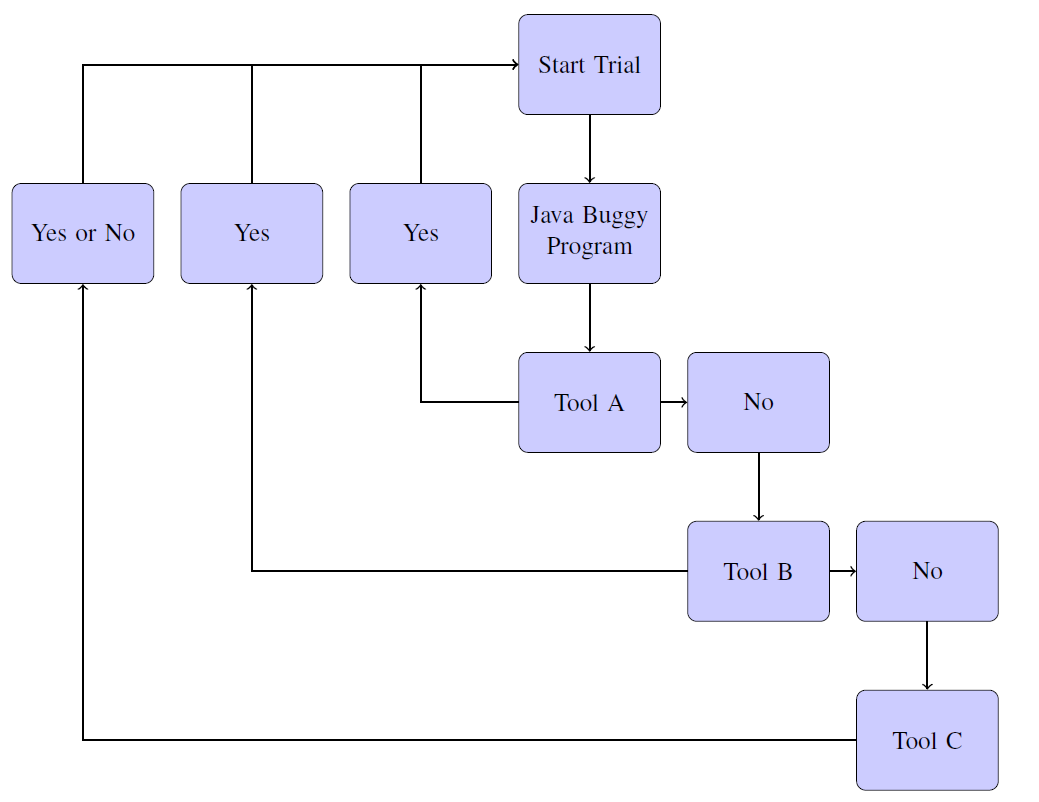
\includegraphics[width=1.15\textwidth]{Methodology.png}
	\end{center}
	\caption{The process of how this empirical study was conducted.}
	\label{fig:metholody}
\end{figure}

Figure 6.1 below displays how each buggy Java program was analyzed. In this study each participant was provided with one of the four buggy Java programs. The order of the Java programs in which the participants performed the analysis was determined by me to prevent any learning effect - meaning that the participants got experience and got better using the tools as they worked through this study. Then the participants were provided with one of the three tools FindBugs, PMD or Checkstyle  - again the tool was determined by me. After the participant had used the first tool to analyze the source code, there were two possibly outcomes. The tool could either have assisted the participant in finding the bug or the bug was not found. If the tool assisted in locating the bug, then the analysis of that Java program was completed and the participant continued by moving on to analyze the next buggy Java program. If the tool was not able to assist the programmer to locate the bug, I determined the next tool for the participant to use. If the second tool was successful in assisting locating the bug, the participant had completed analyzing the program and if not the third tool was provided to the participant. 

This process was repeated for each of the four buggy programs. Each participant had one hour to complete their tasks of analyzing the four programs. 

After the participants had completed the study, a survey was given to them. The survey asked the participants to answer the six questions listed below for each program:
\begin{itemize}
	\item Did you find the bugs?
	\item If yes, did FindBugs assist you in finding these bugs?
	\item If yes, did PMD assist you in finding these bugs?
	\item If yes, did Checkstyle assist you in finding these bugs
	\item Would you use any of these tools in the future for finding logic based bugs?
	\item Suggestion to further improve these tools.
\end{itemize}

The responses from the survey told me results from the study and were used to draw the conclusion.   

I have developed four Java programs each with a bug in its code. The four programs are intended to represent some of the most common mistakes made by Java programmers. I have chosen the bugs based on informal conversations with common students and professors and by searching the Internet. 

The first Java program that was used in this study should convert the numbers ranging from -5 to 32 into the binary representation. The program has a 'for loop' that contains an iteration of the numbers from -5 to 32. However, when participants ran the program, they learned that the program would output the binary representation of the number 33. It is because there is a bug with the 'for loop' in the code. Having a semi-colon right before the program block, will cause the 'for loop' to continue to iterate through the loop without going to the code inside the block. The semicolon was misplaced, as it should not be there at all.

The second Java program calculated the velocity and velocity squared by getting the kinetic and mass as input. As long as mass is not equal to zero the program should run properly, since division with zero is not possible. The program will print out 4 lines. The first and second line will display the kinetic and mass given as input. The third line will display the calculated velocity squared and the last line will display the calculated velocity. The output for velocity squared is incorrect because the equation used in the calculation is incorrect. In the source code the equation is as follows
\begin{lstlisting}
velocity_squared = 3 * (kinetic / mass);
\end{lstlisting}
This equation is incorrect. The equation in the Java source code to calculate velocity squared correctly should have been the following:
\begin{lstlisting}
velocity_squared = 2 * (kinetic / mass);
\end{lstlisting}
The bug in this program is the incorrect number used to calculate the velocity squared.
 
 
 The third Java program takes a text file as input. The file includes a list of airlines that are collaborating so miles can be transferred from airline to another. For example, miles can be  transferred from Air Canada to Ocean Air. However, that is not possible when running the program. The bug is in the canRedeem() method. In the very first 'if' statement, when two strings of current and goal are compared, the '==' operator is used. This is incorrect and the .equals() method should be used instead. The '==' operator checks whether the references to the objects are equal, and the .equals() method checks for the actual contents of the string.
 
 The last Java program was a program of the game  tic-tac-toe. The game was set to a difficult level so the only outcome of the game was either the computer was winning or the game ended in a tie. When the program ran, the output did not display correctly. The bug was in the printBoard() method. In the printBoard() method  a switch statement with 3 cases is used. Both Case 0 and Case 1 need a break statement. However, as can be seen in the source code, there is only a break statement after case 1.

\chapter{Discussion and Results}\label{ch:resultsanddiscussion}

\section{Discussion}

The first Java program that was used for this study calculated the binary of a particular number. FindBugs did not assist any of the participants in finding this bug. Checkstyle was able to detect several warnings in the source code regarding indentation levels. However, it did not further assist programmers in finding this bug. PMD highlighted several lines of the code to give warnings. One of these warnings included the 'for loop' that did not have brackets around it. The semi-colon, may have caused PMD to give this warning and assisted participants to locate logic based bugs in the program.

The second program calculated the velocity squared incorrectly. FindBugs did not assist any of the participants in finding this bug. Checkstyle presented several warnings in the source code regarding indentation level. However, it did not further assist programmers in finding this bug. PMD highlighted several lines of code to give warnings. Unfortunately, it did not assist any of the participants in this study to find the logic based bugs.

The third program used the operator `==' instead of the method .equal(). FindBugs was not able to assist any of the participants in finding this bug. FindBugs detected an incorrect line of source code where an absolute path was declared, however it was not the issue and it was therefore a false-positive. Checkstyle detected several warnings in the source code regarding indentation levels. However, it did not further assist programmers in finding this bug. PMD  highlighted several lines of code to give warnings. Fortunately, it highlighted the specific line of source code that contained the bug. On this specific line, PMD highlights and says to use the .equals() method to compare object references.

In the fourth program, a break statement was missing. FindBugs was not able to assist any of the participants in finding this bug. FindBugs detected an incorrect line in the source code where an absolute path was declared, however that was not the issue and was a false-positive. Checkstyle detected several warnings in the source code regarding indentation level. However, it did not further assist programmers in finding this bug. PMD highlighted several lines of code to give warnings. Fortunately, it highlighted the specific line of source code that contained the bug. On this specific line, PMD highlights and says to use a break statement in a switch case statement. While it appears that PMD seems to be the most efficient bug finding tool in my research, it should be stated that the other tools might prove their strengths in other situations, such as checking the style of how the code is written. 


%SUMMARY:
\section{Results}

Each program was ran by six participants. The tables in this chapter show the result from each participant when using the three tool, including if the three tools were able to assist the participant in finding the bug. 

\begin{table}
\begin{center}
	\begin{tabular}{| l | l | l | l |}
		\hline
		Participant Number & FindBugs & PMD & Checkstyle\\ \hline
		1 & No & Yes & No \\ \hline
		2 & N/A & N/A & No \\ \hline
		3 & No & Yes & No \\ \hline
		4 & N/A & No & No \\ \hline
		5 & No & N/A & No \\ \hline
		6 & N/A & Yes & N/A \\ \hline
	\end{tabular}
	\caption{This is output from all of the participants from Program 1.}
\end{center}
\end{table}


\begin{table}
\begin{center}
	\begin{tabular}{| l | l | l | l |}
		\hline
		Participant Number & FindBugs & PMD & Checkstyle \\ \hline
		1 & No & No & No \\ \hline
		2 & No & N/A & N/A \\ \hline
		3 & N/A & N/A & No \\ \hline
		4 & No & No & N/A \\ \hline
		5 & No & No & No \\ \hline
		6 & No & No & No \\ \hline
	\end{tabular}
	\caption{This is output from all of the participants from Program 2.}
\end{center}
\end{table}


\begin{table}
\begin{center}
	\begin{tabular}{| l | l | l | l |}
		\hline
		Participant Number & FindBugs & PMD & Checkstyle \\ \hline
		1 & N/A & Yes & N/A \\ \hline
		2 & N/A & Yes & No \\ \hline
		3 & No & Yes & N/A \\ \hline
		4 & No & Yes & No \\ \hline
		5 & No & Yes & N/A  \\ \hline
		6 & N/A & Yes & N/A \\ \hline
	\end{tabular}
	\caption{This is output from all of the participants from Program 3.}
\end{center}
\end{table}


\begin{table}
\begin{center}
	\begin{tabular}{| l | l | l | l |}
		\hline
		Participant Number & FindBugs & PMD & Checkstyle \\ \hline
		1 & N/A & N/A & Yes \\ \hline
		2 & N/A & Yes & N/A \\ \hline
		3 & N/A & N/A & No \\ \hline
		4 & N/A & Yes & N.A \\ \hline
		5 & N/A & N/A & No \\ \hline
		6 & N/A & Yes & No \\ \hline
	\end{tabular}
	\caption{This is output from all of the participants from Program 4.}
\end{center}
\end{table}

\newpage
\section{Summary}

FindBugs did not assist the participants in finding any of the bugs in the programs, but highlighted several false positives.

Checkstyle only assisted one of the participants in finding the bug in one of the programs. When Checkstyle was ran for each program, almost every line of source code was highlighted. One of the reasons was the default naming convention. The default configuration of Checkstyle was that certain method names must contain no more than one capital letter. Another contributing factor was using the indentation level. Unlike a programming language such as Python, the source code in Java does not differ if the code is indented or not. If the Checkstyle tool is used for a Python program it would be beneficial in finding bugs because of incorrect indentation.  

PMD was the most useful tool according to the surveys from the participants. The only program where PMD did not assist any of the participants was the second program. In fact, none of the tools were able to assist the programmers in finding the logic based bug in the second program. 

According to the surveys, the end result indicated that the participants would use PMD in the future for finding logic based bugs.

There were multiple suggestions to improve PMD. Several of the participants also suggested improvements to Checkstyle. In the default configuration of Checkstyle, several of the highlighted lines were false positives. Participants suggested to remove most of these warnings since it was difficult to look at the source code when so many false positives were shown. 



%
% $Id: conclusion.tex
%
%   *******************************************************************
%   * SEE THE MAIN FILE "AllegThesis.tex" FOR MORE INFORMATION.       *
%   *******************************************************************
%

\chapter{Conclusion and Future Work}\label{ch:conclusion}

%This chapter usually contains the following items, although not
%necessarily in this order or sectioned this way in particular.



\section{Conclusion}

From the empirical study performed in this senior project, there are indications that the PMD tool best assisted participants in finding logic based bugs. But in all fairness, this study has only scratched the surface of these tools functionality and each of the tools have at least 100 rules/checks that they can perform. FindBugs and Checkstyle do not find as many false positives as PMD and since all tools seemed to work pretty fast, the cost (time wise) of running all three together is small. All three tools are free, so there is neither a financial cost involved in using them. This suggests that all three tools should be used together. I assume it is easier to go through an eventual false positive rather than finding a bug going through the code line by line.
%conclude on goal one
%and goal two

%discussion: what could I have done differently? 
%more bugs could have been analyzed?
%constructed more bugs and run the programs myself?
%used other settings?


%are the tools complementary 

%is the conclusion that a programmer should run all three tools on his code to assist finding errors
%should the conclusion be that a programmer should use all 3 tools to analyze code?

%did any the of tools finds the same errors - 2 of the tools find same error

\section{Future Work}

To make the work done in this senior project more conclusive, the project can be extended. First, more participants could be added to get more reliable results. 

Secondly, the number of programs with bugs could be increased to explore additional logic based bugs. In this project, we have investigated misplaced semi-colon in a for loop, incorrect formulas, incorrect object comparisons, and incorrect placement of break statements in a switch statement. Another logic based bug that could be examined is the order of operation or also known as a operator precedence. For example, if a Java program has two primitive data types of int a = 5 and int b = 8, and should calculate the average by using the following formula: (a + b) / 2. If the parenthesis are not included, the formula will be: a + b / 2. The two formulas calculate different results because of operator precedence, where the first formula is correct for calculating the average of a and b. In the last formula, division is evaluated before addition. 

The three tools examined each has more than 100 different checks and they can be configured to perform the different checks. Different configurations of the tools could be explored including adding programmers own checks. 

The project could also run over an extensive period of time, so participant's long term experience with the tools in an “everyday situation” could be examined.

Another consideration is to evaluate additional tools to explore if there are other tools that are more suited to detect logic based bugs than the tools included in this study.

Lastly, it could be considered to develop a new tool by combining the benefits of the three tools and at the same time minimize the amount of flaws in the tools. 
%Another idea is to evaluate more tools to see if there are tools that are more suited to detect
%logic based bugs. The tools can be used to find other bugs that the bugs that were included in this study.



%   ********************************************************************
%   * IF YOU HAVE ANY APPENDICES (FOR INSTANCE, CODE, DATA, GRAPHS,    *
%   * OR ANYTHING ELSE THAT DOESN'T "FIT" AS REGULAR CHAPTER CONTENT), *
%   * INCLUDE THE FOLLOWING LINE, WHICH INSTRUCTS LATEX TO CHANGE FROM *
%   * NUMBERED "CHAPTER" HEADINGS TO LETTERED "APPENDIX" HEADINGS.     *
%   *                                                                  *
%   * APPENDICES HAVE THE SAME FORMATTING COMMANDS AS CHAPTERS (E.G.,  *
%   * "\chapter{...}", "\section{...}", ETC.)                          *
%   ********************************************************************

\appendix

%
% $Id: appa--code
%
%   *******************************************************************
%   * SEE THE MAIN FILE "AllegThesis.tex" FOR MORE INFORMATION.       *
%   *******************************************************************

\chapter{Java Code}\label{appa:code}
%All program code should be fully commented. Authorship
%of all parts of the code should be clearly specified. 

%   *******************************************************************
%   * SEE THE MAIN FILE "AllegThesis.tex" FOR THE "\lstset" COMMAND   *
%   * THAT DEFINES HOW PROGRAM LISTINGS WILL LOOK.                    *
%   *******************************************************************

%\lstinputlisting{SampleProg.java}
\subsection{Common Java Bug 1}
\lstinputlisting{1/CJB1Final.java}

\subsection{Common Java Bug 2}
\lstinputlisting{2/CJB2Final.java}

\subsection{Common Java Bug 3 and airlines.txt}
\lstinputlisting{3/CJB3Final.java}

\lstinputlisting{3/airlines.txt}

\subsection{Common Java Bug 4}

\lstinputlisting{4/CJB4Final.java}

  % Appendices go here

%   ********************************************************************
%   * THE FINAL COMMANDS DEAL WITH BIBLIOGRAPHY/REFERENCES. IF THERE   *
%   * ARE ANY ITEMS IN YOUR BIBTEX FILE THAT YOU DID NOT REFERENCE IN  *
%   * YOUR PAPER, BUT THAT YOU WISH TO INCLUDE IN THE BIBLIOGRAPHY,    *
%   * YOU MAY SPECIFY "\nocite" COMMANDS TO FORCE THEM TO BE INCLUDED. *
%   *                                                                  *
%   * THE COMMAND "\nocite{*}" FORCES EVERY ITEM IN YOUR BIBTEX FILE.  *
%   ********************************************************************

%\nocite{ckm-acmap-99}   % EXAMPLES OF FORCING THINGS TO BE INCLUDED
%\nocite{Dierckx93}      %   "   "   "
%\nocite{obs-stcav-92}   %   "   "   "
%\nocite{bb4471}         %   "   "   "

\nocite{*} % OR DO THIS TO INCLUDE ALL BIBTEX REFERENCES IN THE BIBLIOGRAPHY

\bibliographystyle{plain}
%\bibliographystyle{bmc-mathphys}
%   ********************************************************************
%   * IF YOU HAVE YOUR BIBLIOGRAPHY IN A SEPARATE ".bib" FILE, HERE IS *
%   * WHERE YOU MUST SPECIFY IT. IN THIS EXAMPLE, THE BIBLIOGRAPHY     *
%   * ENTRIES ARE STORED IN A SUBDIRECTORY NAMED "Bibdir" IN A FILE    *
%   * NAMED "myBibtexDB.bib".                                          *
%   ********************************************************************

\begin{spacing}{1}
\bibliography{Bibdir/myBibtexDataBase}  % File type ".bib" is assumed
\end{spacing}

%   ********************************************************************
%   * THIS FEATURE HAS BEEN DISABLED:                                  *
%   ********************************************************************
% \include{colophon}

\typeout{THEPAGE \thepage}

\end{document}
